\section{Introduction}\label{introduction}
Remaining surgery duration (RSD) prediction supports operating-room
coordination, anesthesia planning, and scheduling, but cases with the
same procedure label can follow different phase orders. This paper asks
whether explicit workflow information improves RSD prediction, and
whether that signal can be estimated from the observed surgical prefix at
inference time. Figure~\ref{fig:paper-overview} summarizes our model: a
ViT-B/16 frame encoder produces visual clip features, while a workflow
token encodes either full-case or prefix-inferred phase-order information
before temporal prediction.
\begin{figure}
\centering
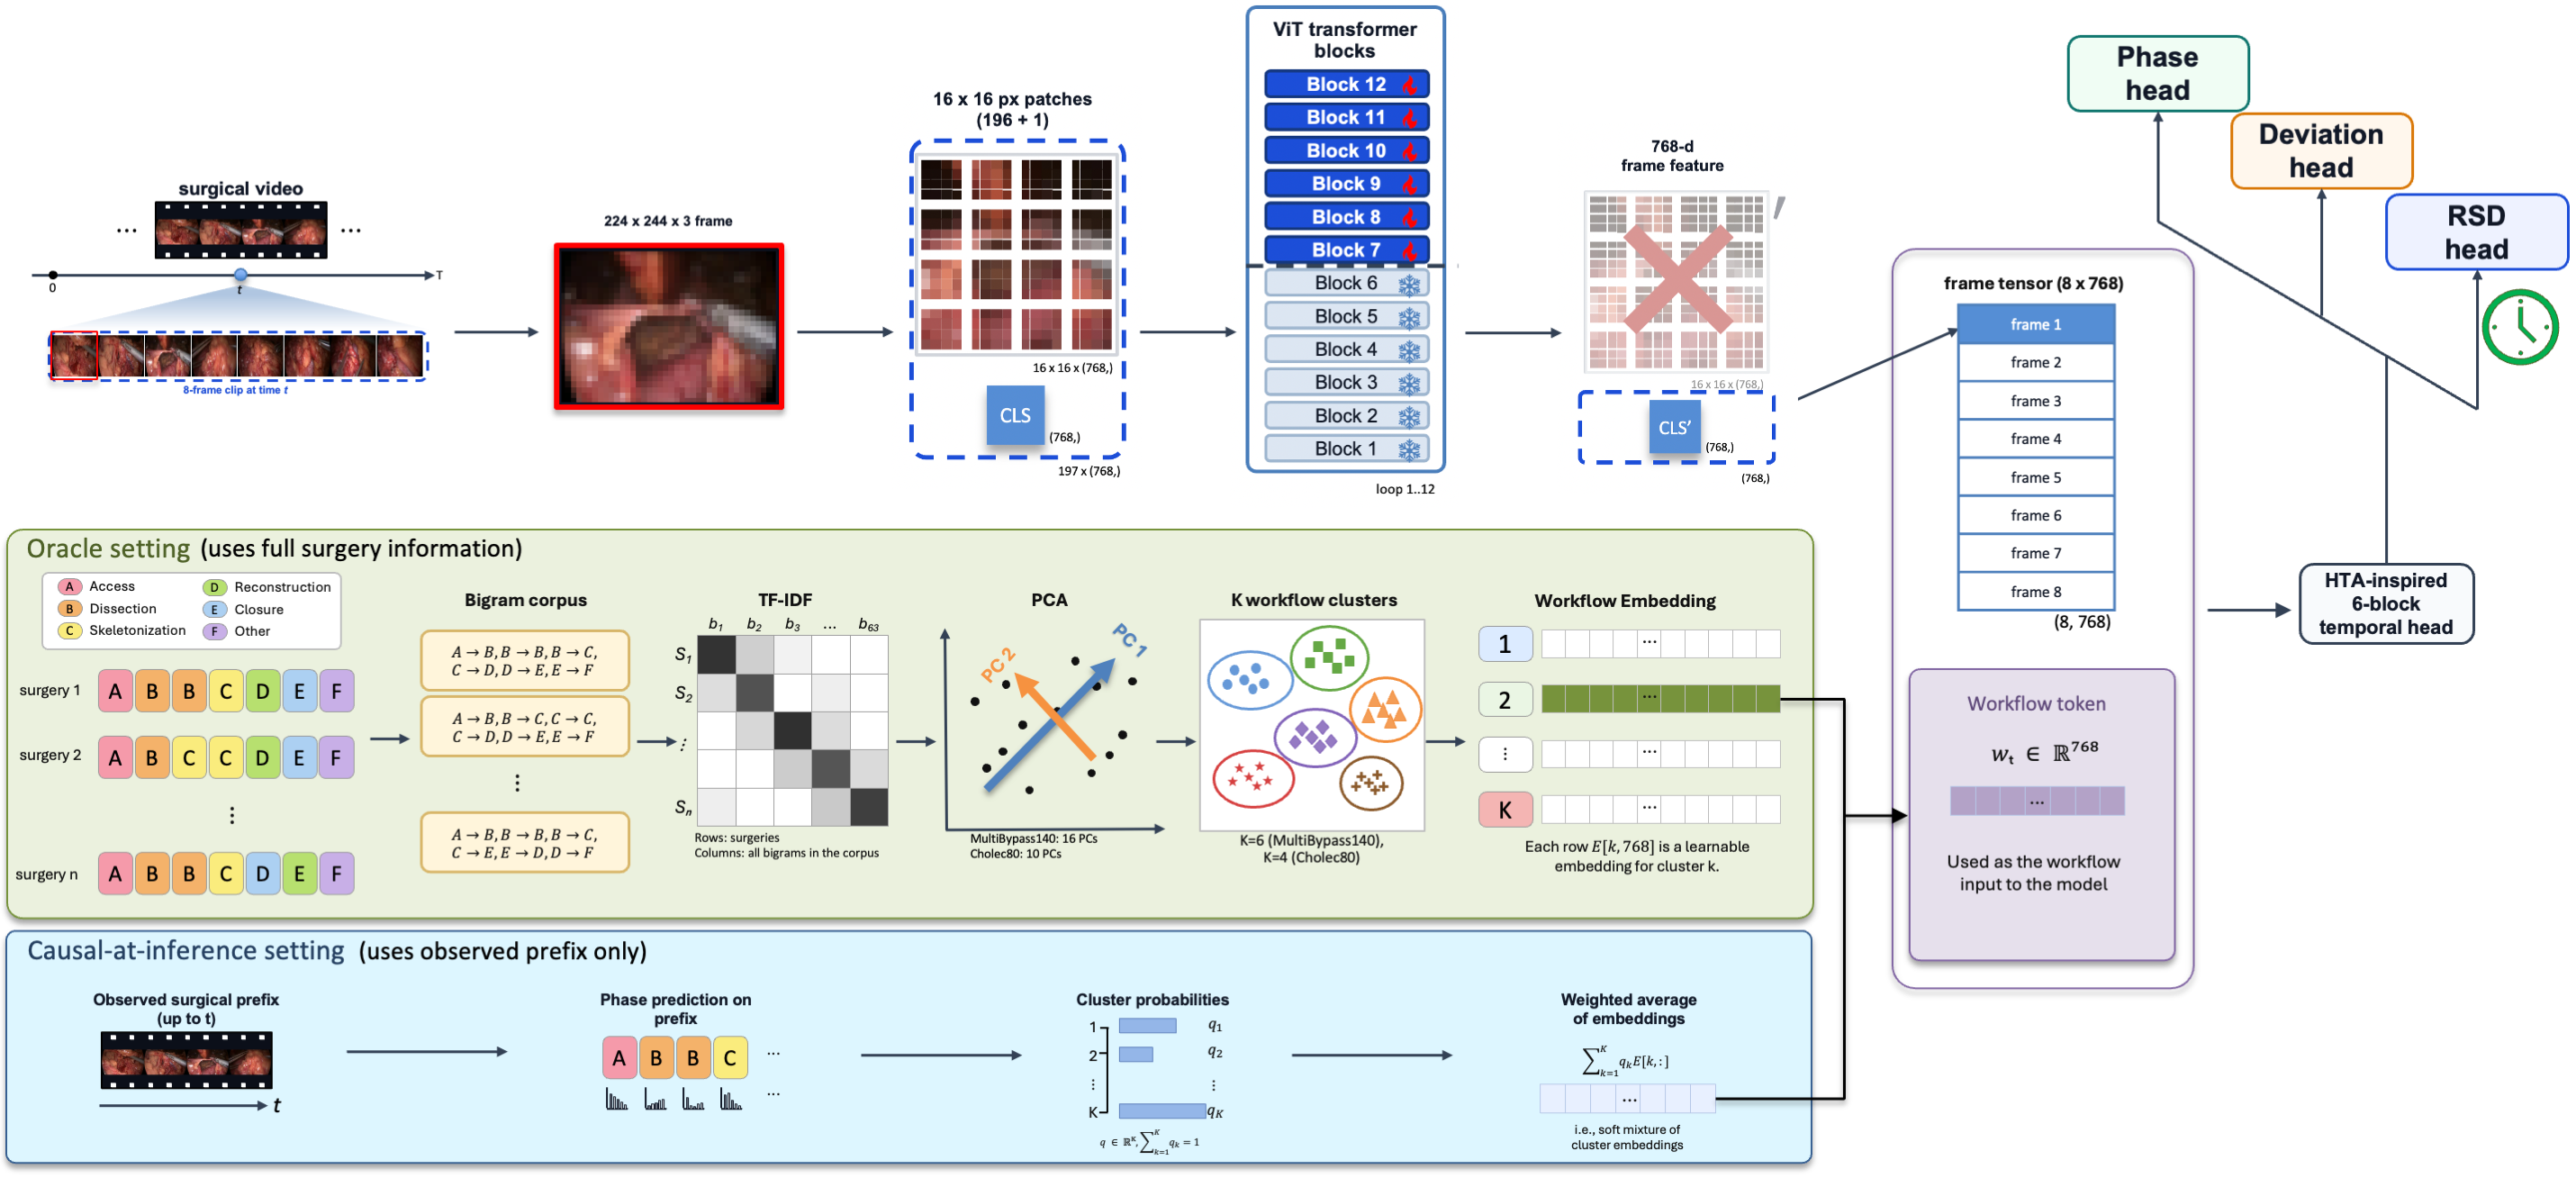
\includegraphics[width=0.98\linewidth,height=0.45\textheight,keepaspectratio,alt={Overall project pipeline for workflow-conditioned remaining-surgery-duration prediction. A real MultiBypass140 clip is encoded by ViT-B/16 into an 8 by 768 frame-feature tensor, combined with a workflow token derived either from full-case phase sequences or prefix-predicted phases, passed through an HTA-inspired temporal head, and evaluated across MB140 and Cholec80 regimes.}]{figures/figure_1_overall.png}
\caption{Overall project pipeline. A surgical video is sampled into an
8-frame clip, encoded framewise by ViT-B/16, stacked into an
\(8 \times 768\) frame-feature tensor, and combined with a workflow
token before the HTA-inspired temporal head predicts RSD, phase, and
deviation outputs.}
\label{fig:paper-overview}
\end{figure}
\subsection{Model and workflow signals}\label{our-approach}

As shown in Figure~\ref{fig:paper-overview}, we use a ViT-B/16 +
HTA-inspired predictor to isolate the effect of workflow conditioning and
protocol design, rather than to propose a new model architecture. Each
8-frame clip is encoded framewise into an \(8 \times 768\) feature
tensor, combined with a workflow token, and passed to a temporal head
that predicts RSD, phase, and deviation outputs. Here, workflow
information means the overall course of the surgery, especially the
sequence of major operative phases. We compare two ways of supplying
that signal:

\begin{enumerate}
\def\labelenumi{\arabic{enumi}.}
\item
  \textbf{Oracle (retrospective) workflow conditioning.} A
  workflow-cluster identifier computed from each video's full phase
  sequence is fed to the model as an input token. This signal uses
  post-hoc knowledge of the entire surgery, which is unavailable during
  a live case; it is therefore a \textbf{diagnostic upper bound} on what
  workflow conditioning could achieve if workflow identity were known
  perfectly. We also report a \textbf{decoupled-oracle} variant: it uses
  the same full-sequence workflow token for RSD prediction, but computes
  the auxiliary phase head from visual features before workflow-token
  mixing. This prevents the phase head from reading the privileged
  oracle token while preserving the oracle workflow signal as a
  diagnostic input to the RSD pathway.
\item
  \textbf{Causal-at-inference workflow conditioning.} At inference, the
  trained model uses its own phase classifier to estimate the phase
  sequence over the \emph{observed prefix} of the surgery, runs that
  estimate through the same TF-IDF/PCA/k-means pipeline used offline,
  and produces a soft cluster posterior. This posterior is converted
  into a soft mixture of the K learned cluster embeddings and used as
  the workflow token. \textbf{No ground-truth phase labels or full-case
  workflow labels are touched at inference; the workflow token is a
  function of model predictions from pixels.} The strict prefix-only
  protocol removes future visual frames as well; the centered-window
  legacy protocol is retained only as a caveated comparator in the
  evaluation branch of Figure~\ref{fig:paper-overview}. Training still
  uses privileged phase/workflow supervision, so we use the term
  \emph{causal-at-inference} rather than \emph{fully causal}, following
  standard usage in the imitation-learning and offline
  reinforcement-learning literatures.
\end{enumerate}

\subsection{Evaluation regimes and protocols}\label{datasets-and-evaluation-protocols} 

We evaluate on two deliberately contrasting benchmarks.
\textbf{MultiBypass140} contains 140 laparoscopic Roux-en-Y gastric
bypass videos, split evenly between Bern and Strasbourg, with 14 phase
labels per video \citep{lavanchy2024multibypass}. Its two-center
structure supports both within-center validation and Bern-to-Strasbourg
train-val transfer. \textbf{Cholec80} is a single-center laparoscopic
cholecystectomy benchmark \citep{twinanda2017endonet}; we use the 72
videos with public phase annotations, split 36/6/30. Because its phase
order is much more standardized, Cholec80 serves as the low-variability
contrast case.

The experiments vary along three axes: dataset/center split, clip
protocol, and workflow signal. We evaluate three regimes: within-center
MultiBypass140, cross-center MultiBypass140, and Cholec80. The
within-center MB140 headline uses fold 0 with 3 seeds; because fold 0 is
the development fold, we also report a 5-fold \(\times\) 3-seed
extension in Appendix C.1. The cross-center MB140 regime trains on Bern
and validates on Strasbourg, using 3 seeds. The Cholec80 regime uses the
36/6/30 split as a standardized contrast benchmark.

For clip construction, the \textbf{strict prefix-only} protocol ends each
8-frame clip at the prediction timestamp and is used for
deployment-relevant claims. The \textbf{centered-window} protocol
attaches the target to the middle frame, so later frames may be visible;
we keep it only as a legacy retrospective comparator. Table~\ref{tab:experiment-matrix} summarizes the experiment matrix.

\begin{table}[t]
\centering
\scriptsize
\setlength{\tabcolsep}{2pt}
\caption{\textbf{Experiment matrix.} Summary of the center splits,
protocols, workflow-conditioning settings, and run sources used in the
paper.}
\label{tab:experiment-matrix}
\begin{tabular}{@{}>{\raggedright\arraybackslash}p{0.14\linewidth}>{\raggedright\arraybackslash}p{0.17\linewidth}>{\raggedright\arraybackslash}p{0.11\linewidth}>{\raggedright\arraybackslash}p{0.22\linewidth}>{\raggedright\arraybackslash}p{0.12\linewidth}>{\raggedright\arraybackslash}p{0.18\linewidth}@{}}
\toprule
Regime & Center / split & Protocol & Conditions compared & Seeds & Source \\
\midrule
MB140 within-center headline & Fold-0 train/val split within MB140 & Strict prefix-only & no-token; retrospective oracle; decoupled-oracle & 3 & Run 033 \\
MB140 5-fold extension & All 5 MB140 CV folds & Strict prefix-only & no-token; retrospective oracle; decoupled-oracle & 5 folds $\times$ 3 (45 runs) & Run 033 (fold 0) + Runs 038--040 (folds 1--4) \\
MB140 cross-center & Train Bern, validate Strasbourg & Strict prefix-only & no-token; retrospective oracle; decoupled-oracle & 3 & Run 034 \\
MB140 cross-center legacy & Train Bern, validate Strasbourg & Centered-window & teacher-forced prefix (3 seeds); historical no-token comparator (1 seed) & 3 / 1 & Run 028 + historical comparator \\
Cholec80 contrast & 36/6/30 split; fold-0 val & Centered-window & no-token; retrospective oracle; teacher-forced prefix & 3 & Runs 017/016/024 \\
Cholec80 strict check & Same 36/6/30 split & Strict prefix-only & no-token; retrospective oracle; teacher-forced prefix & 1 (seed 42) & Runs 046/046b \\
MB140 semantic control & Fold-0 train/val split within MB140 & Strict prefix-only & shuffled workflow token vs. Run 033 no-token/oracle references & 3 & Run 037 + Run 033 refs \\
Pixel-only causal evaluation & MB140 fold 0 (within-center) and Bern $\rightarrow$ Strasbourg (cross-center) & Strict prefix-only & prefix-inferred soft workflow token from model phase predictions; 3 seeds $\times$ 2 regimes = 6 evaluated checkpoints & 3 & Run 035 + Run 044 baseline \\
Posterior-temperature ablation & MB140 fold 0 best checkpoint (Run 033 decoupled seed 42) & Strict prefix-only & soft-cluster posterior temperature sweep ($\tau \in \{0.01, 0.05, 0.1, 0.5, 1.0\}$) on 1 fixed checkpoint & 1 (seed 42) & Run 041 \\
\bottomrule
\end{tabular}
\end{table}

\subsection{Contributions}\label{our-contributions}
The paper makes four contributions. First, we show a consistent pattern across three setting: workflow information helps on the more workflow-diverse MultiBypass140 benchmark, remains useful under cross-center transfer,but provides little or no benefit on the more standardized Cholec80 benchmark. Here, workflow information refers to the overall course of the surgery, especially the sequence of the major operative phases. Second, we compare a real-time evaluation setting that uses only past frames with a legacy setting that also includes future frames, and show that the real-time setting reveals stronger workflow-conditioning gains. Third, we run a control experiment in which workflow labels are randomly reassigned to the wrong surgeries. Under this mismatch, the gain disappears, showing that the improvement comes from correct workflow-conditioning information rather than from merely adding a learnable workflow token to the model input. Fourth, we test a more realistic deployment setting in which the model must infer the workflow signal from the video seen so far, rather than receiving it from the full surgery. In this setting, part of the workflow-conditioning gain remains.

\section{Related Work}\label{related-work}

\textbf{RSD prediction.} \citet{twinanda2019rsdnet} introduced
\textbf{RSDNet} with the self-supervised target \(y_t = (T - t) / T\)
over a CNN-LSTM backbone, reporting $\approx$ 8 min on Cholec80.
\textbf{TransLocal} \citep{loukas2024translocal} augments a CNN-LSTM front-end
with a Transformer using windowed local attention and reports 7.10 min
on the canonical 40-video Cholec80 test split.

The closest prior ideas are \textbf{\citet{kostopoulos2025prediction}} and \textbf{\citet{yengera2019unsupervised}}. Kostopoulos et al.~split videos into long and short cases by \emph{case duration} and use separate random-forest predictors. This differs from our approach because their groups are defined by the
final case length, not by phase-order patterns, and because they switch
between separate models rather than condition one model on workflow
information. Yengera et al.~use unsupervised temporal segmentation as an auxiliary
training task, clustering segments within each video to improve RSD
prediction. In contrast, our clustering operates at the whole-video
level: it uses phase-order bigrams to represent workflow patterns and
feeds that workflow signal to a single RSD model through a learnable
conditioning token.

We are not aware of a published RYGB RSD baseline that evaluates
MultiBypass140 under a cross-center protocol, so MB140 RSD does not
yet have a standardized cross-paper evaluation protocol. Our work is
closest in spirit to RSDNet in treating RSD as the primary task, but
focuses on workflow conditioning rather than temporal-architecture
optimization.

\textbf{Phase recognition.} EndoNet \citep{twinanda2017endonet}
introduced Cholec80 with a CNN phase classifier. Later methods,
including TeCNO \citep{czempiel2020tecno}, Trans-SVNet
\citep{gao2021transsvnet}, SKiT \citep{liu2023skit}, and Surgformer
\citep{yang2024surgformer}, advanced temporal modeling for surgical
phase recognition. We adopt an HTA-inspired temporal head adapted from
Surgformer, train phase classification as an auxiliary task, and reuse
the phase head's predictions to construct the causal-at-inference
workflow signal in \S\ref{inference-causal-at-inference-variant}.


\section{Method}\label{method}

\subsection{Architecture}\label{architecture}

\textbf{Frame encoder.} ViT-B/16 \citep{dosovitskiy2021vit} initialized
from ImageNet-21k via timm (\citealt{wightman2019timm}--present), with the lower 6
of 12 blocks frozen. Each frame is encoded independently; we use the
{[}CLS{]} token's output as the per-frame feature, yielding an
\(8 \times 768\) tensor per 8-frame clip as showing in Figure~\ref{fig:paper-overview}. \textbf{Workflow token.} Each surger
is assigned to one of \(K\) workflow clusters that group videos with
similar phase-order patterns; clusters are built offline by collapsing
each surgery's phase sequence to its ordered phase-transition bigrams,
vectorizing with TF-IDF, reducing with PCA, and running k-means
(\(K = 6\) for MultiBypass140, \(K = 4\) for Cholec80; full
hyperparameters in Appendix B). We represent workflow information with a
learnable embedding table \(\mathbf{E} \in
\mathbb{R}^{K \times d}\), where \(d = 768\). Each row of \(\mathbf{E}\)
is a learned embedding vector that summarizes the procedural pattern of
one workflow cluster, rather than the raw phase sequence itself. In the
oracle setting, the model is given a single cluster label \(z\), and the
workflow token is the corresponding row
\(\mathbf{e}_z = \mathbf{E}[z, :]\). In the causal-at-inference setting,
the model does not know the cluster with certainty: it estimates a
probability distribution \(q\) over clusters from the observed surgical
prefix, and the workflow token is the soft mixture
\(\sum_{k=1}^K q_k \mathbf{E}[k, :]\)
(\S\ref{inference-causal-at-inference-variant}). \textbf{Temporal head.} A
Hierarchical-Temporal-Attention-\emph{inspired} block adapted from
Surgformer \citep{yang2024surgformer} --- not a verbatim reimplementation. Each
of our 6 blocks combines a local-attention branch on the first half of
the 9-token sequence with a global-attention branch over the full
sequence; the published HTA design uses a fuller multi-scale
decomposition that we deliberately simplified for clarity and
reproducibility on this 9-token input. We refer to our block as
``HTA-inspired'' throughout the experimental section. The position-0
output is the global clip representation \(\mathbf{h}_t\). \textbf{Task
heads.} Three MLP heads on \(\mathbf{h}_t\): a 2-layer RSD-regression
head (MSE), a linear phase head (\(P\)-class cross-entropy on the clip's
middle frame), a 2-layer deviation head (BCE with
\(\text{pos\_weight} = 5\) to handle MB140's $\approx$ 2\% positive rate).
\textbf{Multi-task loss} uses \citet{kendall2018multitask}'s uncertainty
weighting: \[
\mathcal{L} = \sum_{k \in \{y, \phi, \delta\}} \exp(-\sigma_k) \mathcal{L}_k + \sigma_k,
\] with learnable \(\sigma_k\). Total parameter count $\approx$ 149.9M, of which
$\approx$ 106.8M are trainable.

\subsection{Inference: causal-at-inference variant}\label{inference-causal-at-inference-variant}

The causal-at-inference variant replaces the oracle's deterministic
cluster lookup with a soft posterior derived from the model's own phase
head over the surgical prefix.

\textbf{At training time.} We use teacher forcing: each clip's
prefix-derived cluster is computed from the \emph{ground-truth} phase
sequence over the prefix \([0, t_{\text{mid}}]\), where
\(t_{\text{mid}}\) is the clip's middle frame. The cluster identifier is
the argmax-posterior cluster from the offline TF-IDF/PCA/centroid
pipeline, with a fallback to the video's full-video oracle cluster on
clips whose prefix contains fewer than 2 unique phases (this affects
\textasciitilde7\% of clips on both datasets; see Appendix A). The
training loss and recipe are otherwise identical to the oracle variant.
We refer to this below as the \textbf{prefix-derived cluster ID}.

\textbf{At inference time.} Given a clip at time \(t\), the model:

\begin{enumerate}
\def\labelenumi{\arabic{enumi}.}
\tightlist
\item
  Forward-passes the prefix frames \(x_{1:t}\) through the visual
  encoder and HTA blocks (using a placeholder cluster identifier; the
  phase-head output is a function of visual features only and is not
  affected by the cluster slot at this point).
\item
  Reads off the phase-head's predicted phase distribution per clip,
  takes the argmax to obtain a predicted phase per clip, and
  concatenates these into a predicted prefix phase sequence
  \(\hat\phi(x_{1:t})\).
\item
  Runs \(\hat\phi(x_{1:t})\) through the same TF-IDF/PCA/centroid
  pipeline used offline, but instead of taking the argmax, computes a
  softmax-of-negative-squared- distance posterior \(q \in \Delta^{K-1}\)
  over the \(K\) centroids. The temperature \(\tau\) of the softmax is a
  single hyperparameter (\(\tau = 0.01\) in our experiments; sensitivity
  in Appendix B).
\item
  Constructs the soft workflow token
  \(\mathbf{e}_z = \sum_{k=1}^K q_k \mathbf{E}[k,
  :]\) and substitutes it into the temporal-head input in place of the
  placeholder token, then re-runs the temporal head and RSD head.
\end{enumerate}

No ground-truth phase labels are provided at inference, and the
workflow token is derived from the observed prefix rather than the full
case. However, one important caveat remains: the underlying clip dataset
is still built as a \textbf{centered window} whose label is attached to
the clip's middle frame. That means the model can still see a few frames
\emph{after} the target timestamp inside the same clip.
Figure~\ref{fig:paper-overview} summarizes where this protocol choice
enters the overall pipeline; the strict protocol ends the visual clip at
the prediction timestamp, whereas the centered-window comparator places
the label at the clip middle.

\section{Experimental Setup}\label{experimental-setup}

All training was on Lambda Cloud GH200 (NVIDIA Grace Hopper Superchip,
96 GB HBM3) nodes in \texttt{us-east-3}, single-GPU per node, 1--4 nodes
used in parallel across experiments via a shared \texttt{bariatric-rsd}
NFS filesystem. The same hyperparameters are used across all training
runs (oracle, no-token, causal) for matched-compute comparison.

\begingroup
\scriptsize
\setlength{\tabcolsep}{3pt}
\renewcommand{\arraystretch}{0.88}
\par\noindent\centering
\begin{tabular}{@{}p{0.33\linewidth}p{0.62\linewidth}@{}}
\toprule
Hyperparameter & Value \\
\midrule
Encoder & ViT-B/16, ImageNet-21k init, 6 lower blocks frozen \\
Temporal head & 6-block HTA, embed dim 768 \\
Clip & 8 frames, stride 5, image size 224 \\
Batch size & 64 \\
Optimizer / schedule & AdamW (lr 1e-4, wd 0.05); cosine annealing over
15 epochs, 5-epoch warmup \\
Mixed precision; gradient clip & \texttt{torch.cuda.amp}; max-norm
1.0 \\
Phase classes (\(P\)); clusters (\(K\)) & MB140: 14 / 6. Cholec80: 7 /
4. \\
Augmentation (train only) & Random resized crop, color jitter, 50\%
h-flip; ImageNet norm \\
Checkpoint selection & Best val MAE across all epochs \\
\bottomrule
\end{tabular}\par
\endgroup
Unless otherwise stated, validation MAE is computed per clip in minutes
and reported as a clip-weighted mean over validation clips, using the
training-set mean duration for denormalization (\(\sim\)110 min for
MB140, \(\sim\)38 min for Cholec80). The deployable evaluation in
\S\ref{strict-pixel-only-causal-deployable-predictor-evaluation} switches
to per-video true-duration denormalization and a video-weighted mean;
Appendix C.2 gives the matched per-video analysis. For reproducibility,
we seed \texttt{torch}, \texttt{numpy}, \texttt{random}, and
\texttt{torch.cuda} from the run's seed argument. We do not enable cuDNN
deterministic mode; empirically, repeated runs vary by about 0.1 min
MAE.

\section{Results}\label{results}

\subsection{MultiBypass140 within-center: workflow conditioning helps under the strict prefix-only
protocol}\label{multibypass140-within-center-workflow-conditioning-helps-under-the-strict-prefix-only-protocol}

We report the headline within-center result on MultiBypass140 fold 0
under the \textbf{strict prefix-only protocol} (the clip ends at the
prediction timestamp, no future frames at inference). The oracle and
decoupled-oracle conditions still consume the full-video cluster ID at
training and inference, so these numbers are clean evaluation results
but are not real-time deployable; the deployable prefix-only causal
evaluation is reported in §\ref{strict-pixel-only-causal-deployable-predictor-evaluation}.

\begin{longtable}[]{@{}
  >{\raggedright\arraybackslash}p{(\linewidth - 6\tabcolsep) * \real{0.2143}}
  >{\raggedleft\arraybackslash}p{(\linewidth - 6\tabcolsep) * \real{0.2857}}
  >{\raggedleft\arraybackslash}p{(\linewidth - 6\tabcolsep) * \real{0.2857}}
  >{\raggedright\arraybackslash}p{(\linewidth - 6\tabcolsep) * \real{0.2143}}@{}}
\toprule\noalign{}
\begin{minipage}[b]{\linewidth}\raggedright
Configuration
\end{minipage} & \begin{minipage}[b]{\linewidth}\raggedleft
Strict val MAE (min, $\downarrow$)
\end{minipage} & \begin{minipage}[b]{\linewidth}\raggedleft
Seeds
\end{minipage} & \begin{minipage}[b]{\linewidth}\raggedright
Source
\end{minipage} \\
\midrule\noalign{}
\endhead
\bottomrule\noalign{}
\endlastfoot
Strict no-token & 13.03 $\pm$ 0.18 & 3 (42, 123, 777) & Run 033 \\
Strict retrospective oracle (full-video phase cluster) & \textbf{12.26 $\pm$
0.09} & 3 & Run 033 \\
\textbf{Strict decoupled-oracle} (token-independent phase head) &
\textbf{12.18 $\pm$ 0.14} & 3 & Run 033 \\
\end{longtable}

\textbf{The strict-protocol within-center workflow-conditioning effect
is 0.85 min --- a 6.5\% reduction over the no-token baseline.} The
decoupled-oracle row is the lowest nominal fold-0 MAE, thought its 0.08 min margin over the standard oracle is within combined seed-level noise ($\approx$0.17 min). It differs from the standard oracle by decoupling gthe phase head from the workflow-cluster token, closing the phase/cluster circularity discussed in Limitations; we adopt this variant primarily to enable the prefix-only causal evaluation.

\textbf{Three signal regimes.} \emph{No-token} receives no workflow
signal; \emph{oracle} receives the full-video k-means cluster ID — a
privileged-information signal (LUPI, \citealt{vapnik2009lupi}) that
serves as a diagnostic upper bound; \emph{decoupled-oracle} uses the
same token but with a decoupled phase head, so the phase logits read
pre-temporal-mixing visual features and the workflow gain cannot be
laundered through the auxiliary head. This decoupled spatial-then-temporal
pattern is standard in surgical-AI multi-task learning (TeCNO,
\citealt{czempiel2020tecno}; MTMS-TCN, \citealt{ramesh2021mtmstcn}); we
adopt it for causal identification, not as an architectural novelty.
Cross-seed variance also drops 3$\times$ under the strict protocol
(strict oracle $\pm$0.09 vs centered-window oracle $\pm$0.33), suggesting
the prefix-only target stabilizes training.

\subsubsection{5-fold cross-validation extension}\label{fold-cross-validation-extension}

To test whether the fold-0 headline generalizes, we ran the
strict-protocol no-token / oracle / decoupled-oracle comparison across
all 5 folds $\times$ 3 seeds (Phase E, 45 runs total). Per-fold mean $\pm$ std
validation MAE in minutes:

\begingroup
\scriptsize
\setlength{\tabcolsep}{3pt}
\renewcommand{\arraystretch}{0.88}
\par\noindent\centering
\begin{tabular}{@{}rrrrr@{}}
\toprule
Fold & no-token & oracle & dec.-oracle & $\Delta$ dec. \\
\midrule
0 & 13.03 $\pm$ 0.18 & 12.26 $\pm$ 0.09 & 12.18 $\pm$ 0.14 & $-$0.85 \\
1 & 11.29 $\pm$ 0.13 & 11.32 $\pm$ 0.29 & 11.07 $\pm$ 0.13 & $-$0.23 \\
2 & 11.60 $\pm$ 0.19 & 11.62 $\pm$ 0.26 & 11.84 $\pm$ 0.14 & +0.23 \\
3 & 10.27 $\pm$ 0.07 & 10.32 $\pm$ 0.11 & 10.39 $\pm$ 0.13 & +0.13 \\
4 & 8.90 $\pm$ 0.22 & 8.67 $\pm$ 0.13 & 8.68 $\pm$ 0.18 & $-$0.22 \\
\textbf{All} & \textbf{11.02 $\pm$ 1.44} & \textbf{10.84 $\pm$ 1.30} &
\textbf{10.83 $\pm$ 1.29} & \textbf{$-$0.19} \\
\bottomrule
\end{tabular}\par
\endgroup

Fold 0 was the development fold, so its larger gain ($-$0.85 min)
reflects in part the standard development/test gap. The 5-fold mean
gain shrinks to \textbf{$-$0.19 min}, with positive $\Delta$ on folds 0, 1,
and 4 and slightly negative $\Delta$ on folds 2 and 3. Per-fold MAE varies
from 8.68 to 13.03 min, indicating substantial case-mix heterogeneity.
We retain fold 0 as the headline (standard practice) and report the
5-fold table for transparency; per-seed numbers in Appendix C.1.

\subsection{Cross-center MultiBypass140: workflow conditioning helps under the strict
protocol}\label{cross-center-multibypass140-workflow-conditioning-helps-under-the-strict-protocol}

We extend the cross-center evaluation protocol introduced by
\textbf{\citet{lavanchy2024multibypass}} for phase and step recognition to the
RSD task: train on Bern's 70 videos, validate on Strasbourg's 70, three
seeds. To our knowledge this is the first cross-center RSD evaluation on
MB140; the training/validation split follows their dataset-paper
protocol. Under the \textbf{strict prefix-only protocol} (Run 034):

\begin{longtable}[]{@{}lrrl@{}}
\toprule\noalign{}
Configuration & Bern $\rightarrow$ Strasbourg val MAE (min, $\downarrow$) & Seeds & Source \\
\midrule\noalign{}
\endhead
\bottomrule\noalign{}
\endlastfoot
Strict no-token & 17.80 $\pm$ 0.55 & 3 & Run 034 \\
Strict retrospective oracle & 17.71 $\pm$ 0.23 & 3 & Run 034 \\
\textbf{Strict decoupled-oracle} & \textbf{17.33 $\pm$ 0.15} & 3 & Run
034 \\
\end{longtable}

\textbf{The strict-protocol cross-center effect is $-$0.47 min}: the same
decoupled-oracle architecture that wins within-center also wins
cross-center, by a smaller but still positive margin. The
decoupled-oracle row is statistically lower than no-token across all
three seeds (17.32, 17.16, 17.52 vs 18.05, 17.03, 18.31). This is more favorable than the legacy centered-window protocol
suggested. Under the centered-window protocol
(Run 028, historical), the teacher-forced prefix variant \emph{failed}
cross-center, resulting in 20.19 $\pm$ 0.02 --- 2 minutes worse than the
centered-window no-token comparator at 18.26. Under the strict protocol,
that failure mode is gone: the workflow signal does transfer
cross-center, just with smaller effect than within-center ($-$0.47 min vs
$-$0.85 min).

\subsection{Cholec80: oracle null, teacher-forced prefix
negative}\label{cholec80-oracle-null-teacher-forced-prefix-negative}

\textbf{Centered-window protocol} (3 seeds, fold-0 val on the 6-video
val split):

\begin{longtable}[]{@{}lrrl@{}}
\toprule\noalign{}
Configuration & Cholec80 val MAE (min, $\downarrow$) & Seeds & Source \\
\midrule\noalign{}
\endhead
\bottomrule\noalign{}
\endlastfoot
No workflow token & 4.61 $\pm$ 0.19 & 3 & Run 017 \\
Retrospective oracle & 4.49 $\pm$ 0.14 & 3 & Run 016 \\
Teacher-forced prefix & \textbf{5.03 $\pm$ 0.07} & 3 & Run 024 \\
\end{longtable}

The oracle / no-token gap of 0.12 min is statistically null (within both
conditions' cross-seed std). The teacher-forced prefix variant is
\textbf{0.42 min worse than no-token and 0.54 min worse than oracle} ---
a clean negative result. On a benchmark where 71\% of videos belong to a
single cluster and 61\% follow the same compressed phase order, there is
no real workflow-order signal to extract; conditioning on a
prefix-derived approximation of ``which workflow'' introduces noise and
actively hurts.

\textbf{Strict prefix-only protocol} (1 seed; same architecture and
recipe with \texttt{-\/-target\_position\ last}):

\begin{longtable}[]{@{}lrrl@{}}
\toprule\noalign{}
Configuration & Cholec80 val MAE (min, $\downarrow$) & Seeds & Source \\
\midrule\noalign{}
\endhead
\bottomrule\noalign{}
\endlastfoot
No workflow token & 4.34 & 1 (seed 42) & Run 046 \\
Retrospective oracle & 4.33 & 1 (seed 42) & Run 046 \\
Teacher-forced prefix & 4.26 & 1 (seed 42) & Run 046b \\
\end{longtable}

\textbf{Under the strict protocol, all three Cholec80 conditions
collapse to the same null} (range = 0.08 min, smaller than typical
cross-seed variance). The teacher-forced prefix penalty seen under the
centered-window protocol (+0.42 min) does not reproduce — it was a
future-frame-leakage interaction, not a property of prefix-derived
conditioning. Cholec80 simply does not reward or penalize workflow
conditioning, regardless of how the signal is supplied — consistent
with the cluster-entropy argument in Appendix C ($H(z) = 1.27$ bits,
71\% of videos in one cluster) and with the clinical fact that
laparoscopic cholecystectomy follows a near-fixed phase template.

\begin{figure}
\centering
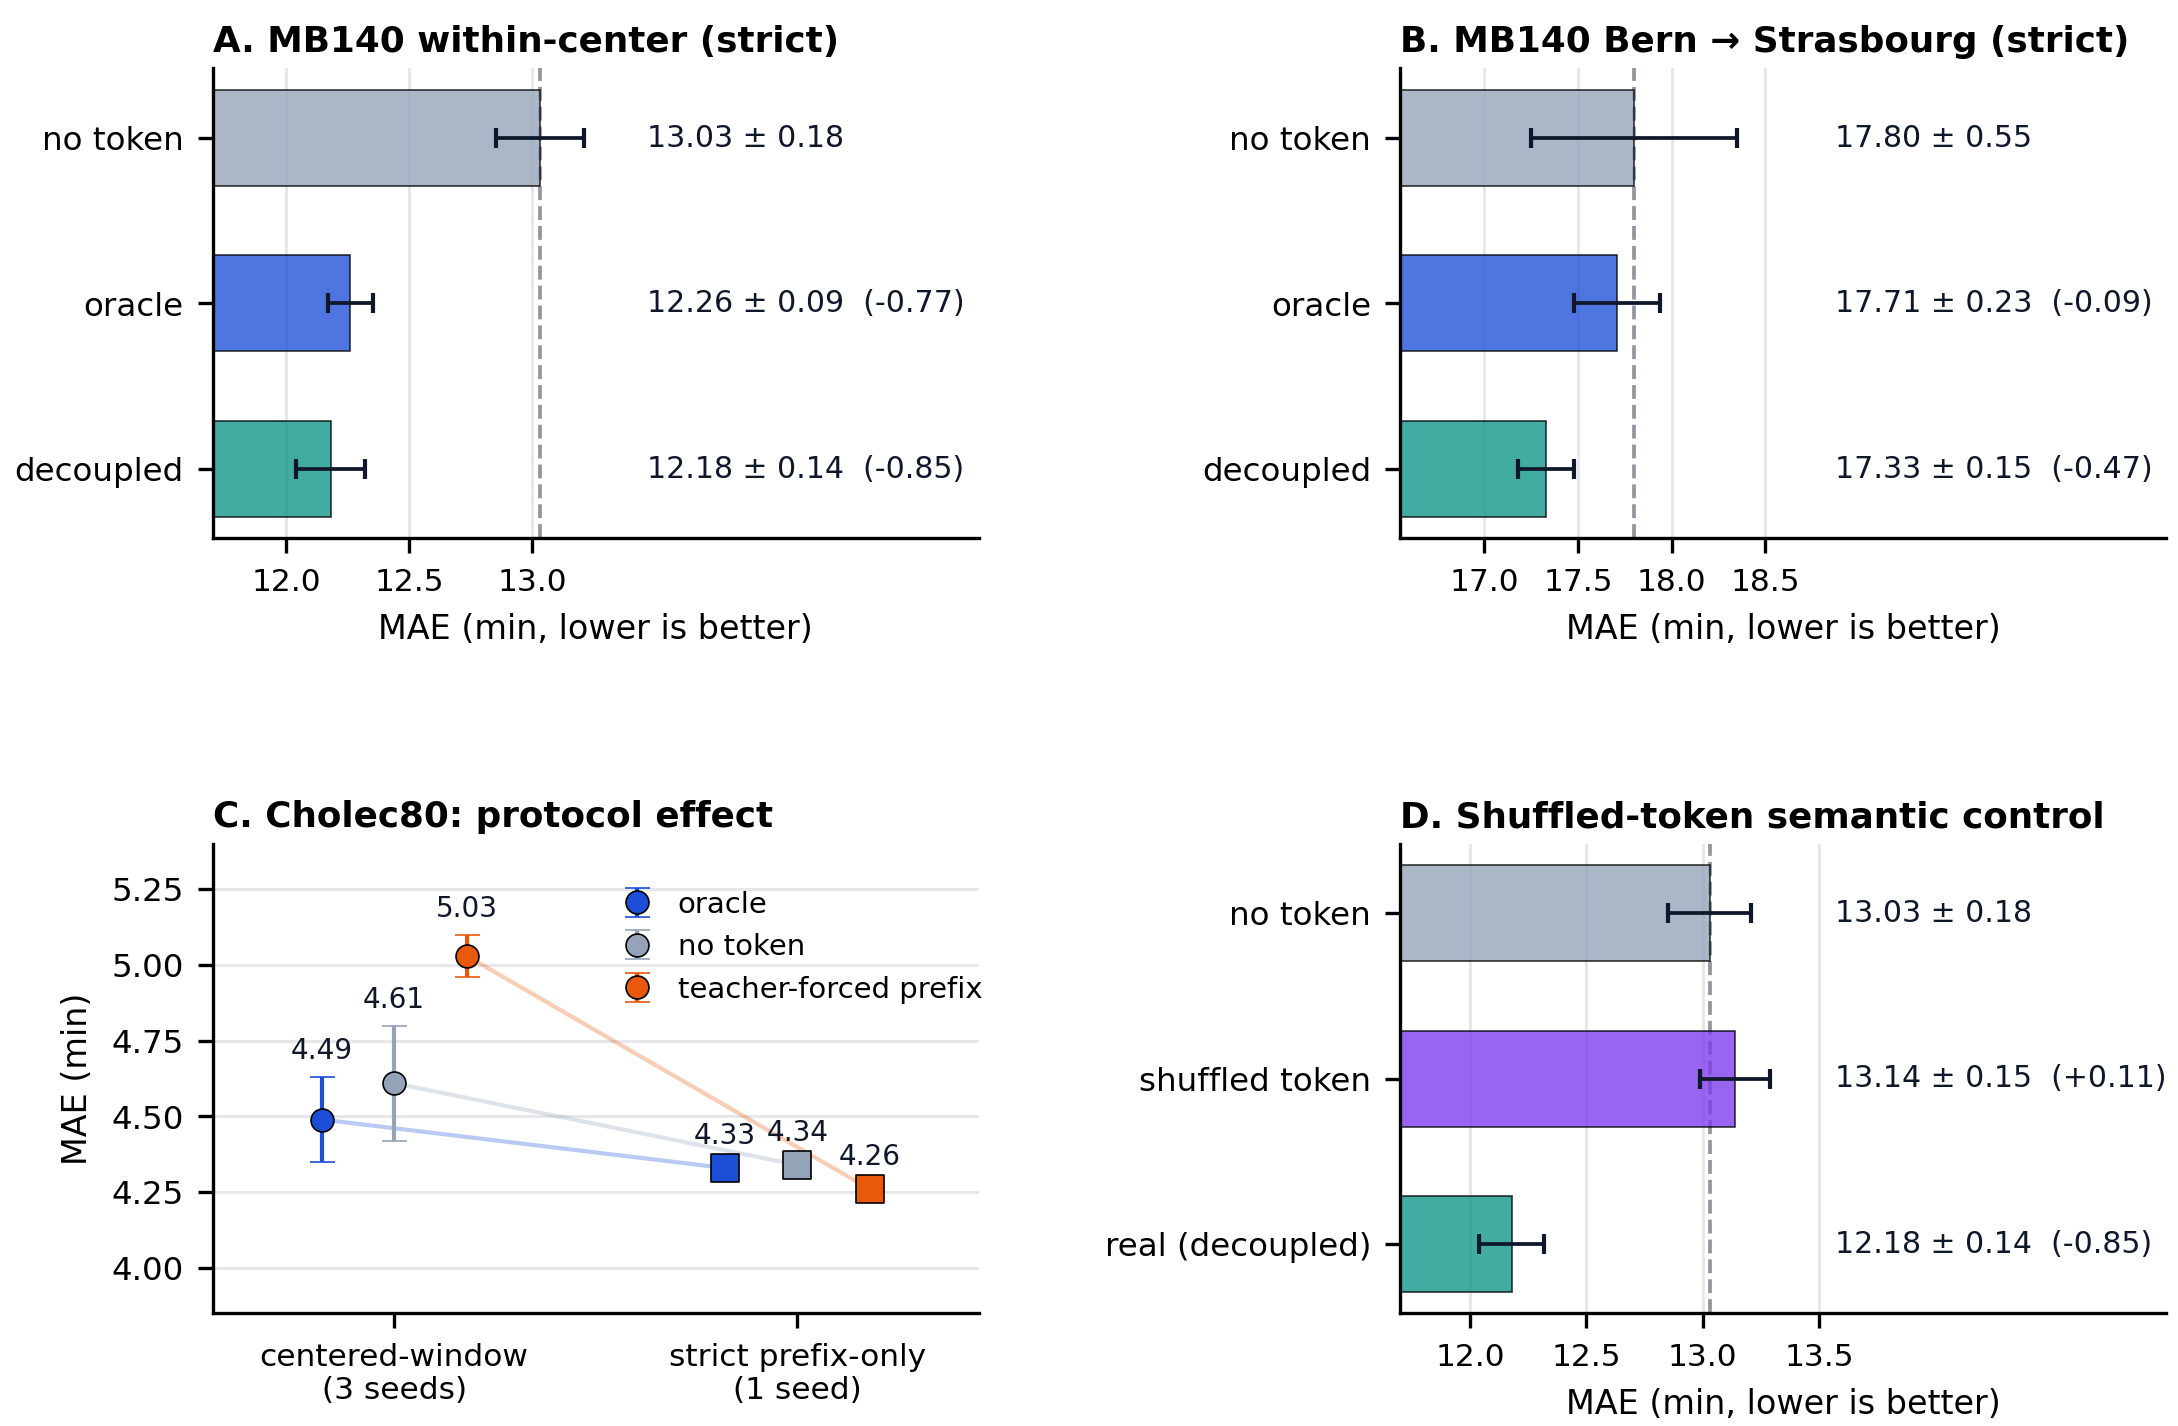
\includegraphics[width=0.8\linewidth,keepaspectratio,alt={Four-panel result summary. Panel A shows MB140 within-center strict prefix-only MAE for no-token, oracle, and decoupled-oracle. Panel B shows MB140 Bern-to-Strasbourg strict prefix-only MAE for the same three conditions. Panel C compares Cholec80 centered-window and strict prefix-only conditions. Panel D shows the MB140 shuffled-token semantic control.}]
{figures/fig2_result_summary_bars.png}
\caption{Main result pattern and controls. (A) On MB140 fold 0 under the
strict prefix-only protocol, decoupled-oracle workflow conditioning
improves MAE by 0.85 min over no-token. (B) The same decoupled
architecture gives a smaller but positive cross-center gain from Bern to
Strasbourg. (C) Cholec80 is the low-variability contrast case: the
centered-window teacher-forced prefix penalty does not reproduce under
the strict protocol. (D) Shuffling workflow tokens destroys the gain,
supporting the interpretation that the token carries workflow meaning
rather than merely adding parameter capacity.}
\label{fig:main-result-pattern}
\end{figure}

\subsection{Strict pixel-only causal: deployable predictor evaluation}\label{strict-pixel-only-causal-deployable-predictor-evaluation}

The strict oracle numbers above all consume the \emph{full-video} oracle
cluster ID at inference. To evaluate a genuinely deployable predictor
--- one that has access only to the prefix at inference time --- we run
the released \texttt{evaluate\_causal\_rsd\_pixel\_only} apparatus
(\S\ref{inference-causal-at-inference-variant}) on the trained Run 033 +
Run 034 checkpoints. At every clip, the
cluster posterior is computed from the model's \emph{own} phase-head
predictions on the prefix, not from ground-truth phase labels.

All numbers in this subsection use a \textbf{uniform metric}: per-video
true-duration denormalization + video-weighted mean. Oracle baselines
are re-evaluated under this metric so the deployable-vs-oracle gap is
comparable; see Appendix C.2 for the matched per-video analysis.

\subsubsection{Posterior temperature is robust}\label{posterior-temperature-is-robust-appendix-b-ablation}

A 5-point sweep of the soft-cluster posterior temperature
\(\tau \in \{0.01, 0.05, 0.1, 0.5, 1.0\}\) on the best within-center
checkpoint (Run 033 decoupled seed 42) yields val MAE in the narrow
range 11.74--11.88 min --- spread 0.146 min, within typical cross-seed
noise. The production setting \(\tau = 0.01\) is essentially optimal. We
report this as a 1-line ablation rather than a separate experiment (Run
041; details in Appendix B).

\subsection{Statistical significance}\label{statistical-significance}

Paired Wilcoxon signed-rank tests on seed-averaged per-video MAE under
the strict prefix-only protocol confirm both headline gains. On
within-center MB140 fold 0 (n=20 videos), oracle beats no-token at
p~=~0.007 (17/20 video-wins, median $\Delta$~=~+0.49 min); decoupled-oracle
vs no-token is at the edge (p~=~0.053, 12/20 wins). On cross-center
transfer (Bern~$\rightarrow$~Strasbourg, n=70), decoupled-oracle reliably beats
no-token at p~=~0.005 (44/70 wins, median $\Delta$~=~+0.39 min). Full
per-comparison tables and 10\,000-sample bootstrap CIs are in
Appendix~C.2.

\section{Discussion and Limitations}\label{discussion}\label{limitations}

\subsection{What the variability-scaling result buys the field}\label{significance-what-the-variability-scaling-result-actually-buys-the-field}

The empirical finding in this paper is one pattern, not one number. As
workflow variability increases, the marginal value of explicit workflow
conditioning becomes more favorable, and the contrast includes both
positive and null/negative cases. On the low-variability side (Cholec80),
conditioning on a teacher-forced prefix signal is
\textbf{+0.42 min worse} than not conditioning at all. On the
high-variability side under the strict prefix-only protocol,
decoupled-oracle conditioning gives \textbf{$-$0.85 min} within-center
MB140 (12.18 vs 13.03 no-token, 3-seed fold-0 val; the full 5-fold
extension averages to \textbf{$-$0.19 min}, with the gain concentrated on
folds 0, 1, and 4 --- see Appendix C.1) and \textbf{$-$0.47 min}
under cross-center transfer (17.33 vs 17.80 no-token), with cross-seed
variance roughly 3$\times$ tighter than the legacy centered-window protocol.
Both the within-center and cross-center decoupled-oracle rows still
consume the \emph{retrospective} oracle cluster ID at inference, so they
constitute clean evaluation results under a deployment-relevant clip
protocol rather than real-time deployable predictions in themselves; the
prefix-only causal evaluator that closes the latter gap is released as
apparatus (\S\ref{inference-causal-at-inference-variant}). The shuffled-token semantic control (13.14
$\approx$ 13.03 no-token, $\neq$ 12.18 decoupled-oracle) verifies that the gain
reflects workflow meaning rather than parameter capacity. The legacy
centered-window fold-0 comparison shows the same direction but a smaller,
only marginal workflow-conditioning trend (Appendix C.4), which is why
the strict prefix-only results carry the deployment-relevant claim.

A concrete consequence for the surgical-video community follows.

\textbf{(1) Benchmark choice has been mis-calibrated.} Cholec80 has
carried phase-recognition and remaining-duration benchmarking for nearly
a decade. Our results show that for the \emph{workflow-conditioning
question} specifically, Cholec80 is the wrong testbed: 71\% of its
videos belong to a single workflow cluster, leaving no residual workflow
signal to learn from. A method designed to exploit workflow variation
will look like a no-op on Cholec80 even when the underlying mechanism is
real on multicenter benchmarks. The community should treat
MultiBypass140, and similar multi-center benchmarks as they become
available, as better current testbeds for this class of question, with
Cholec80 retained as a useful contrast case rather than a primary
leaderboard.

\subsection{Limitations and scope}\label{limitations-and-scope}

\textbf{Protocol scope.} We report two protocols. In the strict
prefix-only protocol (\texttt{-\/-target\_position\ last}), the 8-frame
clip ends at the prediction timestamp; these are the deployment-relevant
numbers. In the legacy centered-window protocol, the clip is centered on
the target frame and may include up to $\approx$ 1 minute of post-target
frames (Figure~\ref{fig:paper-overview}; protocol details in
Section~\ref{datasets-and-evaluation-protocols}); those results are
retrospective comparators, not real-time RSD predictions.

\textbf{Dataset and clinical scope.} MB140 is better suited than
Cholec80 for workflow-conditioning questions, but it is still a
bariatric-surgery benchmark with a largely canonical phase structure.
Workflow clusters are therefore a proxy for the more clinical question
of which operative steps remain and how long those steps typically take,
not a complete representation of surgical difficulty, adhesions,
bleeding, or other deviation events.

\textbf{Oracle and architecture scope.} The pixel-only causal evaluator
removes the inference-time oracle by deriving the workflow token from the
model's own prefix phase predictions, without ground-truth phase labels
or full-video cluster labels at inference. Training still uses
privileged workflow supervision, so the training-time oracle dependency
remains. We also avoid the phase-head circularity in legacy runs by
using a decoupled architecture whose phase logits are read from visual
features before workflow-token mixing.

\section{Conclusion}\label{conclusion}

This paper asked when explicit workflow information improves
remaining-surgery-duration prediction, and answered with a
\emph{variability-scaling} pattern: the value of workflow conditioning
tracks the procedural diversity actually present in the data. Under the
deployment-relevant strict prefix-only protocol, a decoupled-oracle
workflow token reduces validation MAE by \textbf{$-$0.85}~min
(6.5\%) within-center and \textbf{$-$0.47}~min cross-center on
MultiBypass140 (six balanced phase-order clusters, $H(z) = 2.48$ bits),
with the direction confirmed by a 5-fold cross-validation extension;
on Cholec80 (71\% of videos in one cluster, $H(z) = 1.27$ bits), the
same conditioning is statistically null. A shuffled-token control
verifies that the gain reflects workflow meaning rather than parameter
capacity, and the prefix-only causal evaluator --- which derives the
workflow token from the model's own phase predictions, with no
ground-truth phase or workflow labels at test time --- preserves
$-$0.18~min within-center and $-$0.22~min cross-center, supporting
deployable use.

Two consequences for the surgical-video community follow. First, the
strict prefix-only protocol is a methodological lever: it removes a
future-frame-leakage confound that made centered-window cross-center
conditioning look like a $\approx 2$~min failure mode, and it tightens
cross-seed variance roughly $3\times$. Second, Cholec80, the field's
default RSD benchmark, is mis-calibrated for the workflow-conditioning
question; multi-center datasets like MultiBypass140 should carry the
primary leaderboard for this class of method, with Cholec80 retained as
a useful low-variability contrast case. Closing the remaining
training-time supervision gap --- so the deployable predictor matches
the oracle without privileged workflow inputs at training --- is the
natural follow-up.
